\documentclass[11pt,a4paper]{article}

\usepackage[a4paper,margin=1in]{geometry}
\usepackage[T1]{fontenc}
\usepackage{lmodern}
\usepackage{booktabs}
\usepackage{amsmath}
\usepackage{pgfplots}
\usepgfplotslibrary{groupplots}
\pgfplotsset{compat=1.17}

\setlength{\parindent}{0pt}
\setlength{\parskip}{6pt}
\renewcommand{\arraystretch}{1.15}

\begin{document}

\begin{center}
{\Large Numerical Results}\\[0.5em]
{\normalsize 31 March 2026}
\end{center}

\section*{1 \quad Experimental Setting}

\[
S_0 = 100,\quad v_0 = 0.114,\quad v'_0 = 0.110,\quad r = 0,\quad T = 1,
\]
with
\[
\kappa_1 = 5.5,\quad \kappa_2 = 0.1,\quad \theta = 0.078,\quad \xi_1 = 2.689,\quad \xi_2 = 0.502,
\]
and
\[
\delta_1 = \delta_2 = 0.94,\quad \rho_{12} = -0.982,\quad \rho_{13} = -0.727,\quad \rho_{23} = 0.59.
\]

The Bermudan contract is sampled at \(12\) exercise dates. Five strike levels are considered:
\[
K \in \{70,80,90,100,110\},
\]
corresponding to deeper OTM through ITM puts.

All comparisons in this note use the fixed benchmark references generated with \(1200\) Euler steps. The reference direct prices are
\[
V^{\mathrm{ref}}_{110} = 16.645784,\quad V^{\mathrm{ref}}_{100} = 11.356823,\quad V^{\mathrm{ref}}_{90} = 7.402999,
\]
\[
V^{\mathrm{ref}}_{80} = 4.596899,\quad V^{\mathrm{ref}}_{70} = 2.699339.
\]

For any direct price estimate \(V\) and reference value \(V^{\mathrm{ref}}\), the direct relative error is defined by
\[
\varepsilon_{\mathrm{dir}} = \frac{|V - V^{\mathrm{ref}}|}{|V^{\mathrm{ref}}|}.
\]
The reported confidence-interval width is \(2 \times 1.96 \times \mathrm{SE}\).

The purpose of the study is to compare plain LSMC with the Hybrid LSMC--PDE method under \emph{matched path budgets}. Two matched-path regimes are examined:
\begin{itemize}
\item \(60{,}000\) direct paths for both methods;
\item \(20{,}000\) direct paths for both methods.
\end{itemize}

The Euler step counts are \(24,48,72,96\). The emphasis is on the direct estimator, because this is where the hybrid method displayed its clearest advantage.

\section*{2 \quad Matched 60,000-Path Comparison}

Table~1 summarizes the step counts at which the Hybrid LSMC--PDE method achieves a smaller direct error than plain LSMC when both methods use \(60{,}000\) direct paths.

\begin{table}[h!]
\centering
\caption{Steps at which the hybrid method is more accurate under the matched 60,000-path comparison.}
\begin{tabular}{lc}
\toprule
Scenario & Hybrid better at steps \\
\midrule
ITM put & 48, 72, 96 \\
ATM & 48, 72 \\
OTM put & 48, 72 \\
K = 80 put & 48, 72, 96 \\
K = 70 put & 24, 48, 72, 96 \\
\bottomrule
\end{tabular}
\end{table}

The main feature is that the hybrid advantage is strongest in the middle of the step grid, especially around \(48\) to \(72\) steps.

\begin{figure}[p]
\centering
\begin{tikzpicture}
\begin{groupplot}[
group style={group size=2 by 3, horizontal sep=1.8cm, vertical sep=1.8cm},
width=0.43\textwidth,
height=0.24\textheight,
xmin=22, xmax=98,
ymin=0, ymax=8.5,
xtick={24,48,72,96},
ylabel={Direct relative error (\%)},
xlabel={Euler steps},
grid=major,
grid style={draw=gray!20},
axis line style={draw=black!60},
tick style={draw=black!60},
title style={font=\small},
label style={font=\small},
tick label style={font=\small},
legend style={font=\small, draw=none, fill=none},
]
\nextgroupplot[title={ITM put}]
\addplot[blue, thick, mark=*] coordinates {(24,1.926) (48,0.501) (72,0.837) (96,0.360)};
\addplot[orange!85!black, thick, mark=square*] coordinates {(24,1.966) (48,0.439) (72,0.048) (96,0.081)};
\legend{LSMC, Hybrid LSMC--PDE}

\nextgroupplot[title={ATM}]
\addplot[blue, thick, mark=*] coordinates {(24,2.415) (48,1.232) (72,1.227) (96,0.310)};
\addplot[orange!85!black, thick, mark=square*] coordinates {(24,2.590) (48,0.302) (72,0.216) (96,0.412)};

\nextgroupplot[title={OTM put}]
\addplot[blue, thick, mark=*] coordinates {(24,3.523) (48,1.769) (72,1.363) (96,0.112)};
\addplot[orange!85!black, thick, mark=square*] coordinates {(24,3.731) (48,0.526) (72,0.139) (96,0.449)};

\nextgroupplot[title={K = 80 put}]
\addplot[blue, thick, mark=*] coordinates {(24,5.336) (48,2.870) (72,1.429) (96,0.531)};
\addplot[orange!85!black, thick, mark=square*] coordinates {(24,5.385) (48,1.128) (72,0.287) (96,0.167)};

\nextgroupplot[title={K = 70 put}]
\addplot[blue, thick, mark=*] coordinates {(24,7.760) (48,3.791) (72,2.482) (96,0.437)};
\addplot[orange!85!black, thick, mark=square*] coordinates {(24,7.297) (48,1.906) (72,0.847) (96,0.264)};

\nextgroupplot[title={Reading note}, axis lines=none, xtick=\empty, ytick=\empty]
\node[align=left, anchor=west, font=\small] at (rel axis cs:0.05,0.80) {The hybrid advantage is strongest in the middle of the grid.};
\node[align=left, anchor=west, font=\small] at (rel axis cs:0.05,0.62) {At 60,000 paths, \(48\) and \(72\) steps are the most};
\node[align=left, anchor=west, font=\small] at (rel axis cs:0.05,0.50) {consistently favorable region for the hybrid method.};
\end{groupplot}
\end{tikzpicture}
\caption{Direct relative error under the matched 60,000-path comparison.}
\end{figure}

Table~2 reports representative values at \(72\) steps. This is the most informative point because it lies in the strongest favorable region while avoiding the edge effects of \(24\) and \(96\) steps.

\begin{table}[p]
\centering
\caption{Representative metrics at 72 Euler steps under the matched 60,000-path comparison.}
\begin{tabular}{lcccccccc}
\toprule
& \multicolumn{4}{c}{LSMC} & \multicolumn{4}{c}{Hybrid LSMC--PDE} \\
\cmidrule(lr){2-5}\cmidrule(lr){6-9}
Scenario & Dir. err. & SE & CI width & Runtime & Dir. err. & SE & CI width & Runtime \\
\midrule
ITM put & 0.837\% & 0.080321 & 0.314858 & 1.18 s & 0.048\% & 0.026208 & 0.102736 & 238.75 s \\
ATM & 1.227\% & 0.069157 & 0.271095 & 1.25 s & 0.216\% & 0.020668 & 0.081018 & 241.84 s \\
OTM put & 1.363\% & 0.056750 & 0.222460 & 1.16 s & 0.139\% & 0.015294 & 0.059951 & 240.15 s \\
K = 80 put & 1.429\% & 0.044924 & 0.176102 & 1.17 s & 0.287\% & 0.010629 & 0.041668 & 230.58 s \\
K = 70 put & 2.482\% & 0.034333 & 0.134585 & 1.21 s & 0.847\% & 0.006908 & 0.027079 & 233.90 s \\
\bottomrule
\end{tabular}
\end{table}

The direct-error picture is favorable to the hybrid method in the middle of the step grid. The variance picture is even clearer: for every strike in Table~2, the hybrid method has a substantially smaller standard error and a much narrower confidence interval, even though its runtime remains far larger than that of plain LSMC.

\section*{3 \quad Matched 20,000-Path Comparison}

The matched path budget was then reduced from \(60{,}000\) to \(20{,}000\) paths for both methods. This is a more demanding test because both methods receive less Monte Carlo information.

\begin{table}[h!]
\centering
\caption{Steps at which the hybrid method is more accurate under the matched 20,000-path comparison.}
\begin{tabular}{lc}
\toprule
Scenario & Hybrid better at steps \\
\midrule
ITM put & 24, 48, 72, 96 \\
ATM & 24, 48, 72, 96 \\
OTM put & 24, 48, 72, 96 \\
K = 80 put & 24, 48, 72, 96 \\
K = 70 put & 24, 48, 72 \\
\bottomrule
\end{tabular}
\end{table}

Reducing the path budget strengthens the favorable direct-error result. The benchmark LSMC method deteriorates faster than the hybrid method, so the hybrid advantage becomes broader across the step grid.

\begin{figure}[p]
\centering
\begin{tikzpicture}
\begin{groupplot}[
group style={group size=2 by 3, horizontal sep=1.8cm, vertical sep=1.8cm},
width=0.43\textwidth,
height=0.24\textheight,
xmin=22, xmax=98,
ymin=0, ymax=9.5,
xtick={24,48,72,96},
ylabel={Direct relative error (\%)},
xlabel={Euler steps},
grid=major,
grid style={draw=gray!20},
axis line style={draw=black!60},
tick style={draw=black!60},
title style={font=\small},
label style={font=\small},
tick label style={font=\small},
legend style={font=\small, draw=none, fill=none},
]
\nextgroupplot[title={ITM put}]
\addplot[blue, thick, mark=*] coordinates {(24,2.570) (48,1.221) (72,0.773) (96,0.561)};
\addplot[orange!85!black, thick, mark=square*] coordinates {(24,1.468) (48,0.228) (72,0.163) (96,0.407)};
\legend{LSMC, Hybrid LSMC--PDE}

\nextgroupplot[title={ATM}]
\addplot[blue, thick, mark=*] coordinates {(24,4.025) (48,1.336) (72,0.948) (96,1.694)};
\addplot[orange!85!black, thick, mark=square*] coordinates {(24,2.001) (48,0.052) (72,0.475) (96,0.172)};

\nextgroupplot[title={OTM put}]
\addplot[blue, thick, mark=*] coordinates {(24,5.623) (48,2.173) (72,1.788) (96,1.994)};
\addplot[orange!85!black, thick, mark=square*] coordinates {(24,3.118) (48,0.248) (72,0.418) (96,0.253)};

\nextgroupplot[title={K = 80 put}]
\addplot[blue, thick, mark=*] coordinates {(24,7.445) (48,3.193) (72,1.645) (96,1.742)};
\addplot[orange!85!black, thick, mark=square*] coordinates {(24,4.810) (48,0.832) (72,0.012) (96,0.668)};

\nextgroupplot[title={K = 70 put}]
\addplot[blue, thick, mark=*] coordinates {(24,8.911) (48,3.890) (72,1.476) (96,0.748)};
\addplot[orange!85!black, thick, mark=square*] coordinates {(24,6.757) (48,1.589) (72,0.560) (96,1.186)};

\nextgroupplot[title={Reading note}, axis lines=none, xtick=\empty, ytick=\empty]
\node[align=left, anchor=west, font=\small] at (rel axis cs:0.05,0.80) {When the path budget is cut to 20,000, both methods worsen,};
\node[align=left, anchor=west, font=\small] at (rel axis cs:0.05,0.64) {but the benchmark LSMC method deteriorates faster.};
\node[align=left, anchor=west, font=\small] at (rel axis cs:0.05,0.48) {This makes the hybrid advantage more visible across the grid.};
\end{groupplot}
\end{tikzpicture}
\caption{Direct relative error under the matched 20,000-path comparison.}
\end{figure}

\begin{table}[p]
\centering
\caption{Representative metrics at 72 Euler steps under the matched 20,000-path comparison.}
\begin{tabular}{lcccccccc}
\toprule
& \multicolumn{4}{c}{LSMC} & \multicolumn{4}{c}{Hybrid LSMC--PDE} \\
\cmidrule(lr){2-5}\cmidrule(lr){6-9}
Scenario & Dir. err. & SE & CI width & Runtime & Dir. err. & SE & CI width & Runtime \\
\midrule
ITM put & 0.773\% & 0.134824 & 0.528510 & 0.43 s & 0.163\% & 0.045393 & 0.177942 & 76.22 s \\
ATM & 0.948\% & 0.117430 & 0.460326 & 0.46 s & 0.475\% & 0.035909 & 0.140765 & 78.05 s \\
OTM put & 1.788\% & 0.098666 & 0.386771 & 0.50 s & 0.418\% & 0.026674 & 0.104563 & 78.74 s \\
K = 80 put & 1.645\% & 0.076738 & 0.300813 & 0.49 s & 0.012\% & 0.018645 & 0.073089 & 78.68 s \\
K = 70 put & 1.476\% & 0.057802 & 0.226584 & 0.50 s & 0.560\% & 0.012206 & 0.047847 & 78.67 s \\
\bottomrule
\end{tabular}
\end{table}

At \(20{,}000\) paths, the same qualitative conclusion persists and becomes stronger: the hybrid method usually attains lower direct error with much tighter confidence intervals, while the runtime gap remains significant.

\section*{4 \quad Overall Conclusions}

\begin{itemize}
\item The matched-path comparison at \(60{,}000\) paths shows that the Hybrid LSMC--PDE method is most favorable in the middle of the Euler grid, especially at \(48\) and \(72\) steps.
\item The matched-path comparison at \(20{,}000\) paths strengthens this result. When the path budget is reduced, the benchmark LSMC method deteriorates faster than the hybrid method, so the hybrid direct-error advantage becomes broader.
\item In both matched-path regimes, the hybrid method has much smaller standard errors and much narrower confidence intervals than plain LSMC across the full strike range.
\item The main trade-off remains runtime: the hybrid method is much slower than LSMC, even though it is often more accurate and more stable under equal path budgets.
\end{itemize}

Taken together, the experiments carried out on 31 March 2026 support a clear message: when the comparison is made on a fair equal-path basis, the Hybrid LSMC--PDE method performs particularly well at moderate Euler resolutions, and its variance advantage becomes even more valuable when the path budget is tightened.

\end{document}
